%!TEX encoding=UTF-8 Unicode
\chapter{Case Study}
\label{chap:perf}

Optimizing a computational kernel is a complex task, which requires a deep understanding of both the algorithm mechanics and the machine that will execute it.
Simple computational kernels such as matrix multiplication or Cholesky factorization have been subject of years of optimizations, yet some scientists still manage to improve them.
The task is even more complex when it comes to optimizing a whole actual application.
We first need to identify hotspots which means understand where and why the performances are suboptimal.
Then we have to understand their nature and localization both in terms of code and data structure (if they are memory related).
Finally, when optimizing a real life application, it is important to make the code modifications as clear as possible.
Indeed not all developers are specialized in \gls{HPC} and a code is only maintainable if understandable.

\gls{SOFA}~\cite{Allard07SOFA} is a simulation framework designed for exact and interactive physical simulation, it aims at assisting surgeons with real time medical simulation.
Hence  it cannot afford to improve its efficiency by relying on approximations.
Therefore optimizing \gls{SOFA} performance is crucial.
Yet, most of the developers are not from the \gls{HPC} community.
To guide them into this optimization process, we need to analyze the  performances of \gls{SOFA} and identify precisely the hotspots.

In this chapter, we present a case study about the performance optimisation of \gls{SOFA}.
This study case aims at demonstrating the usage of classical analysis tools and emphasize their limits concerning memory related performance issues.
It is organized as follow: first we present \gls{SOFA}, its specificities and previous attempt to parallelize or optimize it in \sect{motivations}.
Then, we discuss the existing profiling tools that can be used to analyze the performances of application in \sect{prof-tools}.
After that we detail our experimental methodology and discuss reproducibility matters in \sect{expe-methodo}.
Finally we present our analysis and first conclusions in \sect{sofa-analysis}.

\section{Motivations}
\label{sec:motivations}

Several efforts were made to parallelize the different part of \gls{SOFA}, using its specificities.
Before discussing these efforts, we need to present more precisely the \gls{SOFA} framework.

\subsection{SOFA: a physical simulation framework}

\begin{figure}[htb]
    \centering
    %!TEX encoding=UTF-8 Unicode

\definecolor{StepCol}{HTML}{4575B4}
\definecolor{ObjACol}{HTML}{FDB863}
\definecolor{ObjAICol}{HTML}{FEE090}
\definecolor{ObjBCol}{HTML}{5E3C99}
\definecolor{ObjBICol}{HTML}{B2ADB2}
\definecolor{ForceCol}{HTML}{ED4049}


\tikzset{
  rounded box/.style={
    shape = rectangle,
    draw,
    rounded corners,
    },
  drawed box/.style ={
    rounded box,
    inner sep=.5em,
    draw = #1,
    },
  ObjA-render/.style ={
      circle,
      shading=ball,
      ball color=ObjACol!80!ObjAICol,
      minimum width=1cm,
  },
  ObjA/.style ={
      circle,
      fill=ObjACol,
      minimum width=1cm,
  },
  ObjB/.style ={
      regular polygon,
      regular polygon sides=8,
      fill=ObjBCol,
      minimum width=1cm,
      minimum height=1cm,
  },
  ObjB-render/.style ={
      regular polygon,
      regular polygon sides=8,
      shading=ball,
      ball color=ObjBCol!80!ObjBICol,
      minimum width=1cm,
      minimum height=1cm,
  },
}

\tikzstyle{StepBox} = [drawed box=StepCol]
\tikzstyle{StepA} = [-latex,StepCol,thick]
\tikzstyle{Force} = [-latex,ForceCol,very thick]

\begin{tikzpicture}[scale=0.74,font=\small]


    \node[ObjA] (Ai) at (0,0) {};
    \node[ObjB] (Bi) at (2,0) {};

    \node[StepBox,fit=(Ai) (Bi)] (init) {};

    \node[StepCol,text width=5em] (inittxt) at (0,1.5) {Initial\\State};

    \node[ObjA] (AI) at (4.5,0) {};
    \node[ObjB] (BI) at (5.5,0) {};

    \node[StepBox,fit=(AI) (BI)] (inte) {};


    \node[ObjA] (Ac) at (8,0) {};
    \node[ObjB] (Bc) at (9.5,0) {};

    \node[StepBox,fit=(Ac) (Bc)] (col) {};

    \node[ObjA-render] (Ad) at (12,0) {};
    \node[ObjB-render] (Bd) at (13.5,0) {};

    \node[StepBox,fit=(Ad) (Bd)] (dis) {};


    % Steps

    \draw[StepA] (init.east) -- node[text width=5em,above=2em]
        {Time\\Integration} (inte.west);

    \draw[StepA] (inte.east) --  node[text width=9em,above=2em]
    {Collision detection\\and response}(col.west) {};

    \draw[StepA] (col.east) -- node[text width=5em,above=2em]
        {Rendering} (dis.west) {};

    \path[StepA] (dis.south) edge[out=-160,in=-20] (init.south) {};

    % Forces

    \draw[Force] (Ai.center) -- ++(.8,0) {};
    \draw[Force] (Bi.center) -- ++(-.8,0) {};

    \draw[Force] (Ac.east) -- ++(-.4,0) {};
    \draw[Force] (Bc.west) -- ++(.4,0) {};


\end{tikzpicture}
% vim: et si sta lbr  sw=4 ts=4 spelllang=en_us

    \caption{The simulation loop.}
    \label{fig:simu-pipeline}
\end{figure}

In \gls{SOFA}, simulation can be seen as a loop depicted in \fig{simu-pipeline}: we start from an initial configuration were a set of objects are subject to a force field.
The second step, called time integration, solves a system of equation to compute the next position of each object.
At that point, some objects might be overlapping.
Thus the third step consist in detecting these overlaps and applying repulsing forces to simulate the collision.
Finally the result of these step is displayed (rendered) and we are back the beginning.
The time integration and the collisions detection are the most costly steps.
Hence many algorithms  were developed to compute them efficiently,  each algorithm being more appropriate for simulating one type of object depending on its form and stiffness.

\begin{figure}[htb]
    \centering
    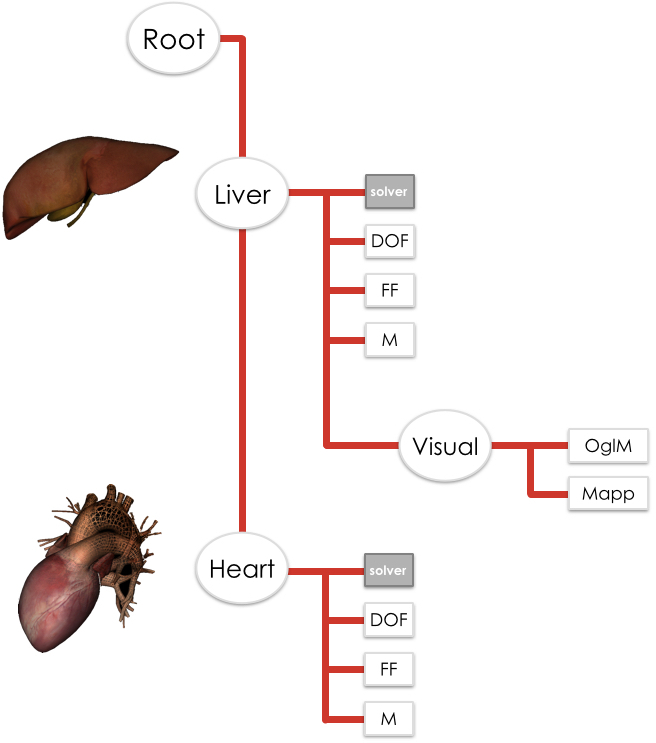
\includegraphics[width=\textwidth]{Sofa-graph}
    \caption[Example of SOFA scene graph.]{SOFA representation of a scene with two objects: a liver and a
        heart. Each node of the scene can embed its own set of solvers and
        visual representations.\\
        Image from SOFA documentation~\cite{SOFA16Sofa}.}
    \label{fig:sofa-tree}
\end{figure}

One of \gls{SOFA} main specificity is that it has a multi-model representation of each component.
A simulation scene is represented as a tree, as shown in \fig{sofa-tree} where each physical object is a node.
Each level of the graph can embed solvers, collision detector and visual representation, overriding the defaults.
This hierarchical representation enable dependencies management between objects and the representation of complex embedded objects~\cite{Nesme09Preserving,Faure11Sparse}.

\subsection{Previous efforts toward SOFA parallelization}

It is important to note that the main developers of \gls{SOFA} are  mostly computer scientists with a physical or medical background but not specialized in \gls{HPC}.
Several efforts were made by external developers to parallelize \gls{SOFA}, most of these efforts consist in optimizing some algorithms which, according to \gls{SOFA} developers, are time consuming.
For instance, Everton Hermann proposed an efficient (sequential) collision detection algorithm based on ray tracing and a parallelization of this algorithm~\cite{Hermann08Raytraced}.
More recently, Julio Toss has been developing several algorithms on \glspl{GPU} to improve the computation time of Voronoi diagrams~\cite{Toss13Parallel,Toss14Parallel}.
Although their computation generates a considerable overhead before the simulation, these diagrams enable efficient simulation of forces propagation in heterogeneous materials~\cite{Faure11Sparse}.
Hence optimizing their computation is critical for \gls{SOFA}.

E. Hermann also proposed a more global approach, exploiting the hierarchy of the scene tree, to parallelize the time integration step~\cite{Hermann09Interactive}.
This parallelization relies on the \gls{KAAPI} runtime~\cite{Gautier07KAAPI} which consider an application as a set of tasks and dependencies between these tasks.
Each task can provide one or several implementations (\gls{CPU}, \gls{GPU} \ldots), the runtime choose online which implementation to use depending on the current performances, which results in portable performances.
With this method, the amount of parallelism depends on the number of objects simulated.
As  most \gls{SOFA} scenes only include a few objects, this parallelization is not suitable for them.

While this approach is more generic it was never actually used by \gls{SOFA} developers for several reasons.
First of all, they are not specialized in parallelism, hence not used to write programs in parallel languages.
Second, \gls{KAAPI} is a research runtime that evolve quickly, maintaining code based on it seemed to costly for them.
Last but not least, while this approach helps to parallelize the code, it does not help finding hotspots and optimizing existing code.
In the end, \gls{SOFA} is currently parallelized using simple \gls{OpenMP} \texttt{\#pragma}.
These  \texttt{\#pragma} are compiler directives to tells the runtime that a region of code should be run in parallel.
While adding such annotation to an existing code is trivial, it requires to spend some time at improving data structures and algorithms to obtain an efficient parallelization.
This method impacts small chunks of code and miss the global aspect of the previous one.
Thus it is considerably less efficient than the \gls{KAAPI} version.

To conclude, it appears that optimizing algorithms or chunk of codes pointed out by \gls{SOFA} developers is not sufficient.
Indeed this approach can miss unknown hotspots and therefore opportunities for optimizations.
Moreover, while the global, runtime based approach seems potentially more efficient than local optimizations, it does not overpass this limitation.
At the end of the day, it appears that identifying precisely unknown hotspots and digging into \gls{SOFA} performances would be more profitable than writing pieces of highly optimized code.

\section{Profiling tools}
\label{sec:prof-tools}

Performance analysis consists of two steps: data collection and presentation.
The first step aims at extracting as much pertinent information as possible from an execution.
Nevertheless, observing an execution is not free: it takes time to count and record events.
As a result, it can impact the application performances or, worst, modify its behavior.
Consequently, any analysis provides a trade-off between the amount of data collected and the impact on the monitored application.
The second step is also challenging as the analysis tool has to to find out which data are pertinent and to present them in a meaningful way to the user.
Many tools were designed to address one or both of these challenges.

Performance counters are dedicated \gls{CPU} registers that were originally designed by vendors to debug their processor prototypes.
They count events such as cache misses, or branch miss-predicts at a very low cost compared to software based solutions.
They can directly be accessed using the \gls{Perf} driver which is part of the \gls{Linux} kernel since version $2.6.31$.
Yet, as a result of their initial aim, the available counters depends of the \gls{CPU} model and vendor.
Furthermore, it requires a deep knowledge of \glspl{CPU} mechanisms to understand the meaning of some counters.
Hence, higher level libraries such as \gls{PAPI}~\cite{Browne00Portable,Malony11Parallel,Weaver13PAPI} and \gls{Likwid}~\cite{Treibig10LIKWID} were designed to make performance counter access and interpretation more convenient.
These libraries provide performance groups and automatically compute comprehensive metrics.
In addition they provide markers that can be used in the code in order to collect counters only during some parts of the execution.
This is useful once hotspots are identified, but can lead to miss a part of the execution if used too early.

An other approach to make performance counters more understandable consists in combining them with contextual informations.
Such informations can be obtained by intercepting libraries calls (system calls, C standard library, \gls{MPI}, \gls{OpenMP} \ldots).
The easiest way to intercept a library call is by overriding it at runtime with the \texttt{LD\_PRELOAD} environment variable\footnote{
    One can use the \texttt{LD\_PRELOAD} environment variable to tell the linker to load a library before running a program.
    As a result, each call to a function from an external library overwritten in the preloaded library will be intercepted.}.
A second method is to rely on binary instrumentation libraries such as \gls{Intel} \gls{Pin}~\cite{Luk05Pin} or Dyninst from the Paradyn Project~\cite{Miller95Paradyn}.
This method is more flexible and usually enable higher level data collection, but it is more intrusive, thus it can impact the behavior of the studied application.
Simulators such as \gls{SimGrid}~\cite{Casanova14Versatile} can be used to overpass these limitations.% still they are usually more complex to install and use.
However \gls{HPC} simulators often focus on explicit communications (via \gls{MPI} or \gls{OpenMP}) discarding the actual computations.
Hence they might miss memory related issues.
Several tools such as \gls{HPCToolkit}~\cite{Adhianto10HPCTOOLKIT}, \gls{PARAVER}~\cite{Pillet95PARAVER}, \gls{TAU}~\cite{Shende06Tau}, \gls{MAQAO}~\cite{Djoudi05MAQAO}, \gls{AMD} \gls{CodeXL}~\cite{AMD16CodeXL} (the successor of \gls{AMD} \gls{CodeAnalyst}~\cite{Drongowski08introduction}) and \gls{Intel} \gls{VTune}~\cite{Reinders05VTune} combines several of these methods to collects traces.

When it comes to presenting performance traces in a readable way, we can split these tools in three groups.
The first ones only provides textual traces and let the user extract pertinent information from them.
It includes the \gls{Perf} driver, \gls{Likwid} and \gls{PAPI} library as well as several \glspl{Pintool}.
Such traces are very useful for small applications as they do not require complex tools to be read.
Moreover they are usually easy to parse and one can build more complex visualization on top of it using \gls{R}, for instance.
Tools from the second group, that includes \gls{VTune}, \gls{CodeXL} tries to present data in a more readable way.
Usually their visualization consist in a set of tables and plots, where they highlight values that seem to be pertinent (for instance cache miss above a fixed threshold) pointing important parts to the user.
Finally, while tools like \gls{MAQAO}, \gls{HPCToolkit} and \gls{PARAVER} propose similar visualizations, but they also provide \glspl{API} to design new visualizations or import external traces.
\gls{Framesoc}~\cite{Pagano13Trace,Pagano14frameSoC} is very similar to the previous tools, the main difference is that it is designed for trace management and analysis.
Consequently it does not provide any way to collect traces but is able to import traces collected by the user.
It describes them with a generic representation and enable easy navigation through different visualizations of the same trace.

To conclude, many tools were developed to monitor the performances of an application.
The best tool depends on the kind of issues we are looking for and the application that is monitored.
Most of the tools discussed here are based on performance counters and thus present data from the point of view of the \gls{CPU}.
In our specific case, we are studying a complex application, yet we are in contact with the developers of \gls{SOFA}.
Consequently they can give us hints about the important parts and the kind of issues we should look for.
Therefore low level tools such as \gls{Likwid} are well suited as they can both compute pertinent metrics and focus on specific parts of the application.

\section{Experimental Methodology}
\label{sec:expe-methodo}

In computer science we can easily monitor our experiments and restart them quickly if something goes wrong.
At the opposite, in other domains, such as biology,  this reactivity is not possible, scientist are forced to write very precise protocols to avoid loosing large amounts of time and money.
By inspiring ourselves from their protocols we could make our experiments reproducible and our research more trustable.

In this section we first introduce reproducibility and how people have tried to reach it in \gls{HPC}, then, we present the methodology we have developed during this thesis to make our experiments as reproducible as possible.


\subsection{Reproducible research}

Measurement bias, which means attributing a consequence to the wrong cause due to an issue in our measurement and analyze method, is a widely known phenomena in scientific communities and is analyzed in most fields.
Mytkowicz et al.~\cite{Mytkowicz09Producing} highlighted several ways to introduce significant measurement bias in computer science experiments without noticing it.
Its experiments showed that measurement bias is both commonplace and unpredictable in our field.
Therefore, the easiest way to deal with this bias is to reproduce studies published by other teams in order to confirm or invalidate their results.
Still, reproducing experiments in computer science and more specifically in \gls{HPC}, is not trivial.

A previous study~\cite{Collberg15Repeatability}, tried to evaluate how reproducible the experiment presented in computer science article are.
To do so, they only focused on the capacity to compile the experimental code and evaluated $601$ articles published in “top ACM conferences and journal”.
From these $601$ articles they were only able to build the environment of $217$ articles.
Moreover it took more than half an hour to build the experimental code of $64$ of these papers and $23$ others required the intervention of the authors.

At this point we need to define precisely reproducibility, for the remaining of this thesis, we will use the definition proposed by Dror G. Feitelson~\cite{Feitelson15From}:

\begin{quote}
    \textbf{Repeatability} concerns the exact repetition of an experiment, using the same experimental apparatus, and under the same conditions.

    \textbf{Reproducibility} is the reproduction of the gist of an experiment: implementing the same general idea, in a similar setting, with newly created appropriate experimental apparatus.
\end{quote}

Repeating an experiment in the sense of Feitelson in \gls{HPC} is nearly impossible.
Indeed repeating an experiment first requires the access to the machine that executed the original one, with the exact same software stack and all the scripts to run it.
Yet, several unpredictable factors can impact the repeatability: between the two experiments, some hardware (for instance a disc) could have been replaced by one faster.
While we can log the whole hardware configuration during the experiment, some other factors, such as the room temperature, can impact the performances and are nearly impossible to measure during the experiment and impossible to reproduce.
Still there is a gap between the definitions of repeatability and reproducibility.
Indeed if we have access to a machine, with the exact same software stack and comparable hardware, as well as the experimental scripts, we can repeat the experiment in \textbf{similar} conditions.
This definition of \emph{similar} repeatability is stronger than reproducibility as we do not re-implement the experiment but re-run it on a similar settings.
Nevertheless we cannot expect the exact same results.
If the experiments compares raw execution times, changing the machine may significantly changes the results, although if we compare relative time (speedup or slowdown) we are more likely to lessen the discrepancy.
Finally, adaptive algorithms may be a limit to similar repetition.
Indeed, small hardware differences might be enough to trigger a change on the executed code of an adaptive algorithm.

Several tools can helps use making experiments more repeatable.
For instance, by running our experiment on a shared platform such as grid5000~\cite{Cappello05Grid5000}, we can argue that other people have access to the same set of machines.
Moreover on these machines, it extremely easy to make a deployable image of our environment.
Using an image provides controls on the installed library, but it is impossible to know or change the version a library without deploying it.
\gls{Kameleon}~\cite{Ruiz15Reconstructable} overpass this limit by describing an environment as a recipe.
It also make the distribution of the environment easier as we only need to distribute the recipe which is a lightweight piece of code instead of an archive containing a whole \gls{OS}.

To reproduce an experiment it is important to understand how it has been designed and how it has evolved from the first version to the results presented in the paper.
Stanisic et al.~\cite[Chapter~4, p31-44]{Stanisic15Reproducible} described an experimental workflow based on \gls{Git} and \gls{Org-mode} to keep track of these evolutions and make easy for anyone to understand it.
One of the main drawback of this workflow is that it is not suitable for experiment generating huge ($\ge$\SI{500}{Mib}) trace files as \gls{Git} is not designed to handle such files.

Many tools were designed to conduct experiments in computer science however they are not designed for \gls{HPC} and using them in our context would require some adjustments.
A comprehensive survey can be found in~\cite[Chapter~3, p17-19]{Stanisic15Reproducible}

\subsection{Experimental workflow}

We design experiments to analyze the behavior of an application, compare it to other applications or to test it under specific circumstances.
The goal of the experiment is to answer a question or confirm an hypothesis.
Answering scientifically a question requires to define:
\begin{itemize}
    \item The environment: the circumstances under which we do the measure.
    In computer science that includes the \gls{OS}, libraries and any user configurations.
    \item The reference cases to which we will compare our results.
        These are usually state of the art existing applications comparable to the one we evaluate.
    \item The inputs given to the tested applications.
    \item The parameters used for each application.
    \item The metrics: a set of quantifiable and measurable indicators used to evaluate our results.
    \item The expected results: what behavior do we expect, what should be considered as abnormal.
\end{itemize}

Designing an experiment consists in translating high level questions into an experimental plan that answers them scientifically.

\begin{figure}[htb]
    \centering
    %!TEX encoding=UTF-8 Unicode

% Layers
\pgfdeclarelayer{background}
\pgfdeclarelayer{bg1}
\pgfdeclarelayer{foreground}
\pgfdeclarelayer{ff}
\pgfsetlayers{background,bg1,main,foreground,ff}

\definecolor{Expecol}{HTML}{B2ABD2}
\definecolor{Analysecol}{HTML}{FDB863}
\definecolor{Resultcol}{HTML}{E66101}
\definecolor{distribcol}{HTML}{5E3C99}

\tikzstyle{distrib} = [drawed box=distribcol]
\tikzstyle{Expebox} = [filled box=Expecol]

\tikzstyle{dep}  = [-latex,Expecol,thick]
\tikzstyle{exec} = [-latex,Resultcol,thick]
\tikzstyle{copy} = [-latex, dashed, thick, Analysecol]

%\newlength{\cornerlength}
%\setlength{\cornerlength}{.1}

\tikzset{
  basic box/.style = {
    shape = rectangle,
    draw,
    text centered,
    text width=6em,
    },
  rounded box/.style={
    basic box,
    rounded corners,
  },
  drawed box/.style ={
    rounded box,
    draw = #1,},
  filled box/.style = {
    rounded box,
    draw  = #1,
    fill  = #1,},
    corner/.style={
      shape=rectangle,
      fill=white,
      alias=this,
      append after command = {
          \pgfextra{
              \begin{pgfonlayer}{ff}
                % Borders of the corner
                \draw [] (this.south west) -- (this.south east);
                \draw [] (this.south west) -- (this.north west);
                \draw [] (this.north west) -- (this.south east);
                % Borders of the main rectangle
                \draw [] (#1.north west)   -- (this.north west);
                \draw [] (#1.north west)   -- (this.north west);
                \draw [] (#1.north west)   -- (#1.south west);
                \draw [] (#1.south west)   -- (#1.south east);
                \draw [] (#1.south east)   -- (this.south east);
              \end{pgfonlayer}
            }
      }
  },
  file/.style ={
      shape = rectangle,
      text centered,
      fill = Expecol,
      minimum height = 5.5em,
      text width = 3.5em,
      append after command = {
            \pgfextra{\let\TikZlastnode\tikzlastnode}
                node [corner=\TikZlastnode, anchor=north east] (corner-\TikZlastnode) at
                (\TikZlastnode.north east){}
          }
  },
  fileA/.style ={
      file,
      fill =Analysecol,
  },
  fileR/.style ={
      file,
      fill =Resultcol,
  },
  header node/.style = {
    %Minimum Width = header nodes,
    font          = \strut\large,%\ttfamily,
  %  text depth    = +0pt,
    fill          = #1,
    text         = white,
    draw},
    header/.style n args={4}{%
    inner ysep = +1.7em,
    append after command = {
      \pgfextra{\let\TikZlastnode\tikzlastnode}
      node [header node=#2,#4] (header-\TikZlastnode) at (\TikZlastnode.#3) {#1}
      %node %[span = (\TikZlastnode)(header-\TikZlastnode)]
       % at (fit bounding box) (h-\TikZlastnode) {}
    }
  },
  hv/.style = {to path = {-|(\tikztotarget)\tikztonodes}},
  vh/.style = {to path = {|-(\tikztotarget)\tikztonodes}},
  fat blue line/.style = {ultra thick, blue}
}
\begin{tikzpicture}[font=\small,scale=.62]

    %expe env
    \begin{pgfonlayer}{foreground}


    \node [Expebox,rotate=90,anchor=west] (configs) at (-3,-2) {Benchmarks, Runtimes, Inputs \ldots};
    \node [Expebox,rotate=90,anchor=west] (venv)  at (-3,2) {Virtual environment};

    \node [fileA](filt) at (0,-3.5) {Parsing script};
    \node [file] (main) at (0,0) {Main script};
    \node [fileA](ana)  at (0,-7) {Analysis script};

    \node [file] (dpl) at (0,3.5) {Launch script};

    \node [Expebox,rotate=90,anchor=north] (mach) at (2,0){Experimental machine(s)};
    \end{pgfonlayer}

    \begin{pgfonlayer}{bg1}
        \node[distrib,fit=(configs) (venv) (ana) (filt) (main) (dpl) (mach),%
        header={Experimental plan}{distribcol}{north}{}] (distenv) {};
    \end{pgfonlayer}

    % Analysis env

    \begin{pgfonlayer}{foreground}
        \coordinate  (inv0)  at (6.5,5.8);
        \node[fileR] (mi)    at (6.5,3.5)  {Meta data};
        \node[fileR] (raw)   at (6.5,0)  {Raw results};
        \node[fileA] (filt1) at (6.5,-3.5)  {Parsing script};
        \node[fileA] (ana1)  at (6.5,-7)  {Analysis script};
    \end{pgfonlayer}

    \begin{pgfonlayer}{foreground}
        \coordinate  (inv1) at (10.5,5.5);
        \node[fileR] (csv)  at (10.5,0) {Filtered results};
        \node[fileA] (ana2) at (10.5,-7) {Analysis script};
        \coordinate  (inv2) at (10.5,-8.5);
    \end{pgfonlayer}

    \begin{pgfonlayer}{bg1}
        \node[distrib,fit=(inv0) (raw) (mi) (filt1) (ana1),%
        header={Raw analysis}{distribcol}{north}{}] (rawa) {};
    \end{pgfonlayer}

    \node[fileR] (res) at (14.5,0) {Human readable results};

    \begin{pgfonlayer}{bg1}
        \node[distrib,fit=(inv1) (csv) (ana2) (inv2),%
        header={Statistical analysis}{distribcol}{north}{text width=5em}] (stata) {};
    \end{pgfonlayer}


    % Paths

    \draw[dep] (configs.south) -- node[color=Expecol,rotate=90,pos=1.3,above=3em] {depends} (main.west);
    \path[dep] (venv.south) edge[out=0,in=180]  (dpl.west);
    % \path[dep] (configs.east) edge[out=0,in=180] node[above] {use} (mach.west);


     \path[exec] (dpl.east) edge[out=-50,in=130]  (mach.north);
     \path[exec] (main.east) edge  (mach.north);
     \path[copy] (ana.east)  edge (ana1.west);
     \path[copy] (filt.east) edge  (filt1.west);

    \path[exec] (mach.south) edge[out=0,in=180] (mi.west);
    \path[exec] (mach.south) edge[out=0,in=180]  node[pos=.9,above=2em,rotate=90] {generate} (raw.west);

    \draw[exec] (raw.east) -- node[pos=.06,below=2em,rotate=90] {generate} (csv.west);
    \path[exec] (filt1.east) edge[out=0,in=180] (csv.west);
    \path[copy] (ana1.east) edge[out=0,in=180] (ana2.west);

    \draw[exec] (csv.east) -- node[pos=.09,below=2em,rotate=90] {generate} (res.west);
    \path[exec] (ana2.east) edge[out=60,in=240] (res.west);

\end{tikzpicture}
% vim: et si sta lbr  sw=4 ts=4 spelllang=en_us

    \caption{Experimental workflow.}
    \label{fig:exp-pipeline}
\end{figure}

\paragraph{Complete experimental plan:}
We consider an experiment as a three steps workflow depicted in \fig{exp-pipeline} determined by a \emph{Complete experimental plan}.
We define the \emph{Complete experimental plan} as the smallest set of scripts and documentation required to repeat an experiment.
It includes the main script that actually run the experiment with all its dependencies.
These dependencies consists in the tested applications (\gls{Git} version, modifications) along with their inputs or the benchmarks used for testing them and the environment on which it is run.
The complete experimental plan also contains the description of the experimental machine(s) and the command(s) or script(s) used to deploy the environment on them and start the main script.
Finally all the scripts used for parsing and analyzing the experimental results are part of the complete experimental plan as they are required to repeat it.
Moreover, designing the analysis at the same time as the experiment help reduce some bias.
Indeed, preparing data presentation before obtaining the actual data forces us to express our expectations.
In the end, if the results do not match theses expectations we are more likely to notice it.

\paragraph{Main experiment:}
The first step of the experimental workflow consist in execution the main experiment on the experimental machines.
This step produces two types of results: the raw results which are the actual output of the experiment and the meta data.
These meta data include all pertinent informations on how the data were produced (information about the environment, commands executed, \gls{Git} version of every applications) and how to interpret them.

\paragraph{Raw analysis:}
We call \emph{Raw Analysis} the second step that extract the raw values needed to compute the metrics defined in the complete experimental plan from the raw results.
This step only aims at reducing the amount of data to analyze (from \SI{100}{Gio} to few Mib in some of our experiments).
The result of the raw analysis is usually one or two \texttt{csv} files that can be easily read by any statistical tool.

\paragraph{Statistical Analysis:}
Finally comes the \emph{Statistical Analysis} which first reads the filtered results and computes statistics such as means, standard error, speedup and slowdown etc.
The second aim of this step is to present a comprehensive visualization of these statistics.

\paragraph{}
While the complete experimental plan is required to repeat the experiment, some people may want to reproduce only the statistical analysis to change it and inspect the results from another point of view.
Furthermore they might want to extract other values from the raw results or get more information about the experimental environment from the meta data.
To enable such partial reproduction we can distribute the \emph{Complete analysis plan} and the \emph{filtered analysis plan} that each includes all the files generate by the previous step and all the files required to redo the next step.
Finally while repeating the whole experiment requires access to the experimental machines, the two last steps are not machine dependent, thus, are easily repeatable.

\subsection{Methodology}

Implementing such an experimental plan is not trivial, we describe here how we design, implement and distribute our plans.

\subsubsection{Construction of an experimental plan}

In \gls{HPC}, an experiment usually consists in evaluating the performances or the correctness of an application or of a tool that uses an application as an input (scheduler, simulator, analysis tool \ldots).
For both we need to find a set of \emph{benchmarks} to conduct our experiments, which means an input representative of the case we want to test.
A benchmark can be either the input of a computational kernel or an actual application used by the tool we evaluate.
%For this need, we use the \gls{npb}~\cite{Jin99NPBOpenMP} as they cover a large set of applications from simple computational kernels to real life applications.
Furthermore if the aim of the experiment is to evaluate the performances of a code that we have developed, we need to test it against existing comparable applications.
Yet, a set of benchmarks might not a sufficient input as such \gls{HPC} applications are often highly configurable.
Thus we must evaluate each program under at least two set of parameters: the default and a tuned version with a set of parameters optimized for the results we are measuring.

Once the benchmarks are chosen, we need to decide on one machine or a set of machines on which we will run the experiment.
This step is crucial as computers architectures are getting more and more complex  and applications are (usually) designed for one type of machines.
Furthermore some tools (such as \gls{Pin}, \gls{PEBS}~\cite{Levinthal09Performance}, \gls{IBS}~\cite{Drongowski07Instructionbased}) are either vendor specific or optimized for some architecture.
Therefore, we often have to repeat the same experiment on several different machines to do a fair comparison.

At this point, we need to find some relevant metrics to answer the questions that we are asking.
These metrics should remain simple as they will be interpreted by humans.
Yet they must also cover every aspects that we are studying.
A complete set of simple measurable metrics is often easier to understand that one complex metric providing an overall score in an unknown unit.
Still simple ratios and percentages can make an analysis more reproducible for instance an execution time is significant only for a very specific configuration on one machine, while speedups and overheads can be compared more easily.

An experimental environment should be \emph{minimalist} yet \emph{sufficient}.
Indeed if the environment is not sufficient we will have to install packages or library before the experiment.
Thus the installed version will depend on the time where the experiment is run, making it almost impossible to repeat.
At the opposite if we include more libraries then we need or worst several version of the same library when it is not required, it might be hard to find out which version was actually used during our original experiment.

Finally it is crucial to write both parsing and analysis scripts before running the experiment.
To do so, we can generate a filler set of (fake) results representing our expectations.
From this set we can design some data visualizations.
Furthermore using this set we can complete the plots with some text describing these expected results.
Such information will stop us from trying to explain a posteriori results that infirm our hypothesis.

\subsubsection{Automation and documentation}

It is crucial that any step of the experiment from the deployment of the environment to the final analysis is properly scripted in a language that can be understood by other developers.
Any manual step can make the experiment impossible to repeat and an obscure code might make it difficult to change some parameters without breaking the whole experiment.

Furthermore, the traces generated by an experiment must be \emph{self explanatory} or at some point they will only be a (large) set of meaningless bytes on a hard drive.
We consider that a trace is \textbf{self explanatory} if and only if we can easily answer the following questions from the raw trace:
\begin{itemize}
    \item How the trace was generated, what is the exact command that launched it ?
    \item What software were used (including their versions and possible modifications) ?
    \item What was the aim of the experiment ?
    \item When was it executed ?
    \item On which machines (description, name and physical location) ?
    \item How are the trace file organized (file hierarchy) ?
    \item How can we interpret these results ?
\end{itemize}
To do so, all our experimental scripts starts the same way: they first create a new directory that will hold the traces.
Then they copy themselves with all the scripts which are on their directory inside it.
After that they duplicate their output to a file in this new directory and log every sensible meta data.
During the experiment, each command is echoed before executing it.
Concerning the data analysis we use \gls{R} as it provides a large set of reliable statistic analysis libraries.
Furthermore thanks to \gls{R-markdown}, we can produce a standalone structured output that contains the original questions, our assumptions, the results and plots, and our observations and comments.
Finally, before distributing an experimental trace, we write a small \texttt{Readme} that explain the file hierarchy and the experiment design (although these informations could be recovered from the meta data and by reading the experiment code).

\begin{centering}
    \begin{minipage}[t]{.48\textwidth}
        \null
        \begin{algorithm}[H]
            \begin{algorithmic}
                \Program{MatAdd}
                    \Function{do\_run}{size}
                        \For{i in $1$..$size$}
                            \For{j in $1$..$size$}
                                    \State C[i][j] = A[i][j]+B[i][j]
                            \EndFor
                        \EndFor
                    \EndFunction
                    \State
                    \Function{Main}{}
                        \For{size in $1$..$N$}
                            \For{run in $1$..$R$}
                                \State \Call {do\_run}{Param}
                            \EndFor
                        \EndFor
                    \EndFunction
                    \State
                \EndProgram
            \end{algorithmic}
            \caption{Dependent runs.}
            \label{alg:dependent-runs}
        \end{algorithm}%
    \end{minipage}
    \begin{minipage}[t]{.48\textwidth}
        \null
        \begin{algorithm}[H]
            \begin{algorithmic}
                \Program{MatAdd}
                    \Function{Main}{size}
                        \For{i in $1$..$size$}
                            \For{j in $1$..$size$}
                                    \State C[i][j] = A[i][j]+B[i][j]
                            \EndFor
                        \EndFor
                    \EndFunction
                \EndProgram
                \Program{Experiment}
                    \Function{Main}{}
                        \For{size in $1$..$N$}
                            \For{run in $1$..$R$}
                                \State \Call{exec}{MatAdd size}
                            \EndFor
                        \EndFor
                    \EndFunction
                \EndProgram
            \end{algorithmic}
            \caption{Independent runs.}
            \label{alg:independent-runs}
        \end{algorithm}
    \end{minipage}
    \vspace{1em}
\end{centering}

To evaluate the variability and reduce the effect of external noise, we run each configuration at least $30$ times.
These runs are all independent therefore we must avoid to make them artificially dependent.
The \alg{dependent-runs} shows a very simple experiment where the runs are launched by the process that actually do the experiment.
As we do not create a new process for every run, some cache effects might appear between the runs improving their performances.
Thus these runs are artificially dependent.
An easy way to avoid this bias is to start a new process for each run, as shown in \alg{independent-runs}.
Yet, this is not enough to protect our experiment from system noise
Indeed if at some point of the experiment a system process (such as \texttt{logrotate}) interfere with our experiment, the performance of a set of runs will drop.
As the runs are executed in order, it might be correlated with the size, and therefore we will not realize that it is due to external noise, and credit the size for it.
While if we randomize the runs, the performance drop will affect several runs (but not all) for different size.
As a result we will observe a high variability for the impacted sizes and therefore conclude that something might have interfered.
To do so, our experimental scripts generate a list of runs that should be executed, shuffle it and then execute them in this randomized order.

Each run consists of three step: a pre-command that can set specific environment values, the actual command that execute the benchmark and the post command that can save and pre-process data, might compute metrics and must restore the normal state.
The first and last steps are not mandatory, yet any environment change must be restored on the last step.
Each of the commands executed by these 3 steps are logged before execution.

\subsubsection{Distribution}

The experimental plan is mostly composed of source code, thus it can easily be distributed using a \gls{VCS}.
As it often depends of external programs, it is preferable to use \gls{VCS} which manage dependencies and patches such as \gls{Git} or mercurial.
We distribute our experimental plans as \gls{Git} repositories, were each dependencies is tracked as a submodule.
This repository includes an initialization script that retrieves all dependencies and apply the patch required.
If the virtual environment is written as a \gls{Kameleon} recipe, it is trivial to distribute it inside the \gls{Git} repository.
Yet in this case, we have to build the image from the recipe during the initialization.
Often the environment is just an archive, in that case, we make it available on a http server, and the initialization script take charge of downloading it.
Finally, we add a Readme describing how to run the experiment, on which machines and what variables should be changed (if any).

Distributing the raw analysis is more difficult as some trace files can be quite heavy and code repositories are usually not designed to handle large files.
Large file hosting services such as Renater File Sender or Zenodo are well suited to upload these files.
Moreover they generate \gls{DOI} that can be used both in the article and in the experimental \gls{Git} to link to the trace.

The statistical analysis could be distributed via code repository or with large file sharing service as it does not include large files.
Yet large file sharing seems more suitable to us as the filtered traces are not code but experimental results.

\section{SOFA Analysis}
\label{sec:sofa-analysis}

In this section, we present first the experiment designed to produce a performance analysis of \gls{SOFA}, then we discuss about the obtained result and the possibility of improvements.

\subsection{Experimental plan}

The current version of \gls{SOFA} is mostly sequential with a simple \gls{OpenMP} parallelization in some places.
Yet this parallelization is known to be often inefficient.
The \gls{SOFA} developers gave us four simulation scenes specifically designed to test the most popular parts of \gls{SOFA}, and hints about functions that are known as hotspots.

We decided to use \gls{Likwid} to analyze \gls{SOFA} performances as it is quite flexible allowing both global (wrapper mode) and local (marker mode) analysis and provides several useful metrics and performance groups out of the box.

More specifically, we focused on the following metrics:
\begin{itemize}
    \item \emph{Idle time ratio}: The CPU is idle when it is waiting for a transfer to memory,  disc or network \glspl{I/O}.
        Idle time can often be reduced either by overlapping it with computation or by improving memory (or \glspl{I/O} access pattern).
        This metric gives the ratio between the time spent idle and the time actually spent computing things during the simulation.
    \item \emph{Simulation time}: The time spent inside \gls{SOFA} simulation loop, this is only useful to compare parallel executions to sequential ones.
    \item \emph{Runtime ratio}: For each function, the ratio of the time spent in this function and the total time spent in the simulation loop.
        This metric highlights functions that are actually hotspots.
    \item \texttt{L2}, \texttt{L3} and \texttt{MEM} predefined groups from \gls{Likwid}.
        These groups mainly compute the data volume exchanged and the bandwidth at their level (respectively second level of cache, third level of cache and main memory).
        These two metrics and more precisely their evolution between sequential and parallel executions tell us how data is shared between the threads and if it is shared efficiently or not.
        These metrics are computed by counting the misses at one level lower (hence the absence of \texttt{L1} group).
\end{itemize}

\begin{table}[t]
    \centering
    \begin{tabular}{lccccc}
        \toprule
        \multirow{2}{2cm}{CPU} & Vendor & Model & Core & Threads & Frequency \\
        \cmidrule(lr){2-6}
        & Intel & Xeon E5-1607 & $4$ & $4$ & \SI{3.00}{Ghz} \\
        \midrule
        \multirow{3}{2cm}{Cache\\and\\Memory} & L1 & L2 & & L3 & Memory \\
        \cmidrule(lr){2-6}
        & \multicolumn{2}{c}{Private} & & \multicolumn{2}{c}{Shared} \\
        \cmidrule(lr){2-3}
        \cmidrule(lr){5-6}
        & \SI{32}{Kib} & \SI{256}{Kib} & &\SI{10}{Mib} & \SI{16}{Gib} \\
        \bottomrule
    \end{tabular}
    \caption{Hardware configuration of Naskapi.}
    \label{tab:naskapi-hw}
\end{table}

As \gls{SOFA} is mainly used on personal machines and not \gls{HPC} ones, we ran our performance evaluation on a recent desktop machine called \emph{Naskapi}.
The hardware specifications of this machine are described in \tbl{naskapi-hw}.
It runs a \gls{Debian} \emph{Wheezy} on a Linux kernel $3.2.0$-$4$ with hyper threading disabled.


The experimental methodology described in \sect{expe-methodo} evolved during this Ph.D thesis, hence the experiments presented here does not fit it perfectly.
Mostly the runs were independent but not randomized, and the experimental logs were not as complete as they should.
Furthermore as \emph{Naskapi} is a desktop machine and not a node from a cluster, we did not deployed an image of the system.
Therefore repeating these experiment in the exact same condition do not seem possible.
Yet we distribute the experimental plan and the trace, which should make the experiment easy to reproduce on github: \url{https://github.com/dbeniamine/Sofa\_expe}.


\subsection{Results and Discussions}

To present the results of our evaluation, we will focus on two \gls{SOFA} scenes that illustrate the kind of results we obtained.
The first scene is called \emph{linearQuadraticFrame}, for this scene the \gls{OpenMP} parallelization provides a speedup of $1.37$ with four threads.
This speedup seems rather low, yet as the parallelization is only partial we need to determine if we can actually reach a higher speedup.
However the second scene \emph{linearRigidAndAffineFrame} has a speedup of $0.87$ which means that the parallel version is slower than the sequential one.
Thus our first goal is to understand why some scenes take advantage of this parallelization while some other are slowed down by it.

Before digging into the differences between these scenes, there are two noticeable similarities between them to discuss.
First the idle time ratio reported by \gls{Likwid} showed that, for the sequential version of the code, during almost half of the simulation the processor is idle, which means that it spend a lot of time waiting for \glspl{I/O} or memory accesses.
In parallel,  this idle time increases.
This behavior is expected as the \gls{OpenMP} based parallelization only affect some small parts of the code, hence as soon as the code is not in a parallel loop, $3$ threads out of $4$ are idle.
Still it means that their is room for improvement even for the sequential version.
The second noticeable similarity is that the functions pointed by the developers only represent around \SI{30}{\%} of the simulation time, which means that there are some unknown hotspots left.

From here, we know that there might be a memory issue (as the processor spend a lot of time idle).
Moreover we have two scenes: one where the parallelization speed the execution up and one on which it slows it down.
We compared the bandwidth and data volume going int each cache level and the main memory for the two scenes and for the functions indicated by the developers.
Those functions are generic and thus their actual code varies depending on the parameters of the simulation.
Therefore while the compared functions are similar in terms of role in the simulation, the manipulated data as well as the executed code is different for the two scenes.

\begin{figure}[htb]
    \centering
    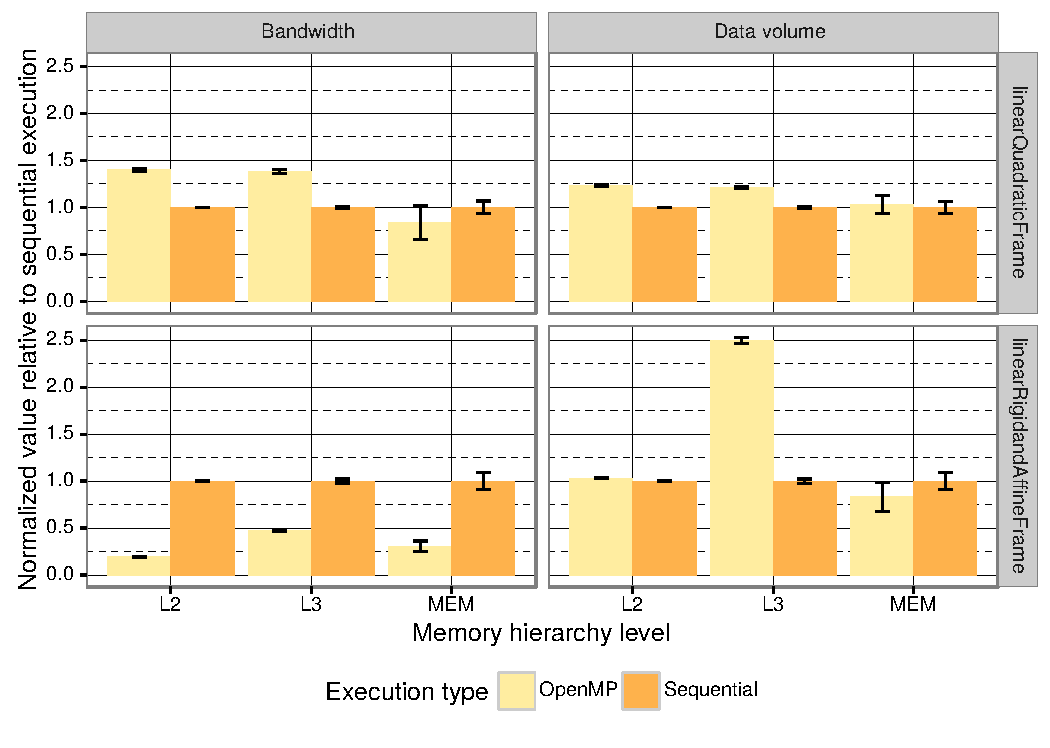
\includegraphics[width=\textwidth]{SOFA_perfctr.pdf}
    \caption[SOFA likwid results.]{Differences of bandwidth and data volume, from L2 cache to main memory, between sequential and parallel execution of \gls{SOFA} on two different simulation scenes.
        \\
        For both bandwidth and data volume, the value is normalized to the mean value of the corresponding sequential execution.
        \\
        For bandwidth, higher is better while for data volume lower is better.
    }
    \label{fig:SOFA-perfctr}
\end{figure}

\fig{SOFA-perfctr} shows the bandwidth (left side) and the data volume (right side) for the two functions (\emph{linearQuadraticFrame} above, \emph{linearRigidAndAffineFrame} below) from \texttt{L2} cache to the main memory.
Each point represents the mean of $60$ runs and the error bars represents the standard error.
To make the plot more readable, we have normalized each value by dividing it by the value for the corresponding sequential run.
Thus these plots show the evolution of the bandwidth and data volume when we use the \gls{OpenMP} version of \gls{SOFA}.

We can see that for the first scene, both the bandwidth and data volume increases by a factor of $1.5$ in the cache and stays comparable in the main memory when we use the parallel version.
This means that there are more useful data in the cache, either because each thread works on a smaller set of independent data which fit in the cache, or because they share data efficiently.
At the opposite, for the second scene, the bandwidth drops down at each level while the data volume stays still except at the \texttt{L3} level where it increases by a factor $2.5$.
It is important to note that the \texttt{L3} cache is the only shared cache of this machine.
It means that several threads are writing the same data, invalidating each other private cache and requiring the coherency protocol to interfere.
This behavior is called false sharing and is a well known performance issue that have been introduced by Torellas et al.~\cite{Torrellas94False}.

At this point we can say that false sharing occurs in this precise function, yet we do not know on which data structure.
We could dig onto the code and try to understand the memory access pattern of each data structure to see where the false sharing does occurs.
By looking at \gls{SOFA}'s code, we can see that the main difference between the two version of the function is that for \texttt{linearRigidAndAffineFrame} there is one more loop in the computations.
Still this code manipulate several data through many indirections.
Therefore determining on which data the false sharing is happening could be extremely slow.
Furthermore this approach is not generic at all.
Once we have done it for one particular function, we would have to redo the same analysis and optimization for each potential hotspot.

Moreover as we have seen with the runtime ratio, this particular false sharing issue only represent a small part of the execution.
Therefore a more generic approach would be welcome.

From that point it seems clear that \gls{SOFA} is having memory performance issues.
Yet, we need a generic tools to analyze its performances from the memory point of view.
Such tool should be able to establish a complete diagnosis of the memory usage.
To do so, this tool need to identify memory access patterns and differentiate the efficient ones from the others.
Moreover to correct an inefficient pattern we need to know precisely why it is inefficient.
Thus this tool should classify them in terms of performance issues.
Finally it needs to localize these patterns which means determine where it occurs in term of data structure, which thread(s) are responsible for the accesses and to what lines of code it correspond.
To sum up, this ideal tool will trace every memory access of an application and give to the user a list of inefficient patterns.
For each pattern it will specify very precisely what kind of issue is occurring, where it happens and how we could fix it.


% vim: et si sta lbr  sw=4 ts=4 spelllang=en_us
